La presente sección consiste en la presentación de la solución escogida
para mejorar la problemática de las pequeñas empresas para competir en lo
referente a comercio electrónico con sus pares mayores.

\section{Metodología de la solución}
\label{sec:4.1}

La idea para dar solución a la problemática de las micro empresas,
que consiste en atraer y retener clientes, para así poder competir
con empresas de mayor tamaño, tiene como base el uso de una herramienta
OpenSource, para así crear una tienda virtual atractiva a los usuarios
y que pueda estar a la altura de grandes sitios web.

Las siguientes características son necesarias para poder implementar un sistema
web enfocado a una pequeña empresa, que no posee los recursos necesarios
para un gran despliegue web:

\begin{itemize}
    \item {\bf Bajo costo:}
        Debido al bajo capital que poseen micro o pequeñas empresas,
        ésta característica es bastante crucial.
        La poca viabilidad de utilizar soluciones completas ofrecidas
        por empresas externas, nos lleva a poder utilizar una o más herramientas
        que en su conjunto emulen a un sistema completo que necesita ser
        implementado.

    \item {\bf Facilidad de configuración:}
        Existen diversas herramientas que ayudan a un negocio emergente a crear
        una web, pero pocas están pensadas para ser configuradas por un usuario
        sin tantos contenidos tecnológicos.
        Esta característica es vital, pues como ya mencionamos,
        se necesita una personas con los conocimientos necesarios tanto
        de instalación como configuración, los cuales pueden ser solucionados
        con la contratación de una persona externa.

    \item {\bf Facilidad de administración:}
        Característica clave dentro de la solución planteada.
        El sistema sera administrado, la mayoría del tiempo, por el dueño de la
        empresa, el cual debe ser capaz de hacer tareas en el sistema
        de manera rápida y frecuentemente, por lo que un grado
        de complejidad en términos de administración jugarán en contra
        a la hora de poder aprovechar el sistema a disposición.
        Adicionalmente, se necesita un sistema de administración rápido,
        para evitar estar mucho tiempo realizando una tarea simple, que
        además de conocimientos del sistema, pueden ser provocados por sistemas
        que no poseen una implementación de funcionalidades ordenadas.

\end{itemize}

Una vez creada la tienda virtual, la empresa entra a competir electrónicamente,
pero en desventaja, con empresas de mayor capital y por ende con tiendas virtuales
de mayor tamaño y que utilizan conceptos para atraer y retener a los clientes.
Para poder competir directamente, es necesario utilizar estos mismo conceptos para
poder alcanzar, de cierta forma, el nivel de visitas y ventas de estos grandes
sitios web.

Para poder disminuir la brecha entre la solución propuesta y una tienda virtual
de gran tamaño utilizaremos el concepto de {\GAM}.
Esta idea ayudará a la tienda a atraer y retener clientes con la utilización
de conceptos del desarrollo de juegos, que ya se han mencionado en éste documento,
de los cuales se han seleccionado los siguientes elementos, como parte
de un esquema clave a implementar. Estos ya han sido utilizados y probados en diversos
sistemas como herramientas para motivar al usuario\cite{SocialMotivation}

\begin{itemize}
    \item {\bf Puntuación:}
	Este estilo de recompensa es uno de los primeros creados como parte de
	implementar gamification. Es una de las formas mas sencillas de empezar
 	a utilizar gamification\cite{OnlineComp} y de la cual se pueden basar otros tipos de recompensas.

        En el contexto de nuestra solución, esta herramienta consiste en la entrega de
	puntos por la realización de tareas definidas, como:

    \begin{itemize}
        \item Inscripción:
            Esta tarea otorga al usuario 500 puntos.
        \item Comentarios en productos:
            Otorga 100 puntos por cada comentario, con un máximo de 5 comentarios
            con premio.
        \item Compras realizadas:
            Se le premia con un 10\% de la compra en puntos.
    \end{itemize}

        Estos puntos son equivalentes a crédito en la tienda y pueden ser
        utilizados como parte de pago.
        Estos son utilizados para que los clientes vuelvan a comprar a la tienda,
        utilizando créditos generados por él mismo.


    \item {\bf Achievements (logros):}

	Esta forma de motivación, a travez de la entrega de medallas o \emph{achievements}
	ha empezado a ser utilizada para manejar el comportamiento de los
	usuarios dentro de la web\cite{BehaviorBadges}.

        Dentro de la solución se implementara la entrega de medallas (\emph{achievements})
	coleccionables entregados a los clientes por cumplir con tareas definidas, como:

        \begin{itemize}
            \item Inscribirse.
            \item Primer inicio de sesión.
            \item Primer comentario/reseña.
            \item Primera orden completada.
            \item Compra por una suma mayor a \$15,000 CLP.
        \end{itemize}

        Esta recompensa es utilizada con el fin de entregar la sensación de éxito,
        e importancia en entre otros compradores y así mantener una motivación
        de seguir comprando y su estado dentro de la comunidad.

    \item {\bf Referals (Referencias):}
        Invitaciones de usuarios de la tienda que son entregadas a posibles
        clientes para que estos conozcan y compren en la tienda.
        Esta herramienta entrega un beneficio mutuo tanto al que hizo la invitación
        como al invitado. Esta recompensa es un cupón de descuento de 500 puntos.
        En primer lugar el usuario invita a un cliente no suscrito en la tienda
        enviando un cupón valido por 500 puntos.
        Luego, este al comprar con este cupón reenvía,
        proceso interno, un cupón de 500 puntos al usuario que lo invito.
        Esto es utilizado para atraer clientes con gustos similares
        a la tienda, pues el usuario que entregue invitaciones, lo hará a su
        grupo cercano, y así sucesivamente.

\end{itemize}

Al unir la tienda virtual con las ideas propuestas dadas por {\GAM} se crea un
sistema de ventas online capaz de competir con las características similares del
comercio electrónico de tienda que poseen más capital y experiencia en este ámbito,
pero que estas aun implementan otras herramientas que la ayudan aun mas.

\section{Selección de sistema}

Como parte de la investigacón, se tubierón que seleccionar distintos sistemas web para
crear una tienda electronica, estos son \emph{Magento}, \emph{Prestashop}, \emph{Wordpress
$+$ Woocommerce}.

Para poder elegir entre estos sistemas, se proponen las siguientes métricas para
la selección:

\begin{itemize}

    \item Facilidad de instalación:
        Esta métrica muestra el nivel de conocimientos que se debe
        tener para poder realizar una instalación completa y exitosa del sistema.
        También demuestra que tanta ayuda existe durante la misma (comentarios,
        ejemplos, etc).
        Ésta se medirá con una escala de 1 (lo más fácil) a 10 (lo más difícil).

    \item Facilidad de administración:
        Escala que mide el nivel de conocimientos para poder utilizar el
        \emph{dashboard} de administración de cada sistema.
        También se toma en cuenta la ayuda y ejemplos que da el sistema al usuario.
        Esta medida en una escala de 1 a 10, siendo 1 el mas fácil y 10 el mas
        difícil.

    \item Actualizaciones y comunidad activa:
        Métrica que demuestra que tan periódicamente se realizan actualizaciones
        al sistema.
        También mide la comunidad que existe tras cada proyecto tanto en tamaño
        como en actividad.
        Esta escala también se mide entre 1 y 10, siendo 1 una periodicidad baja
        de actualizaciones y falta de comunidad y 10 actualizaciones diarias y
        una comunidad altamente activa y colaboradora.

    \item Características utilizables:
        Mide la existencia de plugins que implementen herramientas de {\GAM}
        y si estas son gratuitas o de pago.
        Si son de estas últimas si son de bajo o alto costo.

    \item Traducciones:
        Muestra si existe una traducción del sistema a otros idiomas, en especial
        al español.

\end{itemize}

En el siguiente cuadro~\ref{tab:comp_tools} muestra la comparación de los tres
sistemas preseleccionados para implementar la solución propuesta.

\begin{table}[h]
\footnotesize
\setlength\extrarowheight{5pt}
\begin{tabular}{p{2.5cm}|p{1.8cm}|p{2.5cm}|p{2.8cm}|p{2.5cm}|p{2cm}|}
                        & Dificultad\newline Instalación
                        & Dificultad\newline Administración
                        & Actualizaciones y\newline Comunidad
                        & Características\newline Utilizables
                        & Traducción \\ \hline

Magento                 & 7 & 8 & 3 & Si,\newline Alto costo & Parcialmente \vspace{0.2cm} \\
Prestashop              & 6 & 7 & 4 & No                     & Si    \vspace{0.2cm}\\
Wordpress +\newline Woocommerce & 4 & 5 & 7 & Si,\newline Gratuitas\newline Bajo costo\newline Alto Costo & Si
\end{tabular}
\caption{\cmf{Falta caption}}
\label{tab:comp_tools}
\end{table}
\section{Herramientas}

Para implementar la solución propuesta se necesitó el uso de variadas herramientas.
En un principio éstas serían desarrolladas específicamente para realizar las
tareas requeridas pero luego de investigar el estado del arte de estas tecnologías
se tomo la decisión de utilizar herramientas ya disponibles que tuviesen
características similares a las requeridas en donde su modificación requeriría
menos tiempo que el desarrollo completo de estas.
Otra característica que ayudo al cambio de paradigma fue que en todas las
herramientas a utilizar existe una comunidad altamente activa que da soporte y que
llegaría a ser útil al momento de configurar o modificar alguna de estas.

La base del sistema utilizado es Wordpress, por ser uno de los
CMS~\footnote{Content management system o Sistema de gestión de contenidos}
más famosos, y ampliamente utilizado\cite{CmsPerformance}.

Esta herramienta permite crear una web para manejar contenidos de una forma fácil,
tanto la instalación como la administración de las funcionalidades básicas del sistema.

Wordpress posee una fase de instalación sencilla debido a que los recursos
necesarios son pocos. Se necesita poseer un \emph{hosting} donde alojar el sitio y
dominio, además de una base de datos relacional, como MySQL o postgres.
Una gran ventaja de esta herramienta es que al necesitar recursos básicos,
servidor web y base de datos relacional, puede ser instalado de manera fácil en la
mayoría de los \emph{hostings} a nivel mundial.
Una vez instalado, la administración total del sistema es relativamente simple,
ya que posee un \emph{dashboard} con todas las opciones necesarias
tanto para la configuración inicial del sistema, como para la modificación
de algunas características importantes, desde el contenido, hasta el tema
y diseño del sitio.

La características principal de Wordpress, que ha ganado mediante
la comunidad detrás del proyecto, es la variedad de plugins, que
tienen tanto un proceso de instalación fácil, como su administración,
la cual sigue los mismos principios de administración de Wordpress.
Dichos plugins, son el elemento distintivo de cada CMS
y en nuestro caso, han sido los actores principales para aplicar
todos los elementos de {\GAM} en el sistema web.

\cmf{Si este es el snapshot para mostrar el "Tema" utilizado,
no creo que nadie querría usar el sitio. Saca un screenshot bonito
del sitio completo, no importa que use una página completa. Qué
es la pifia que se vé al lado derecho? como que cortaste una columna?}

\begin{figure}[!htb]
  \centering
  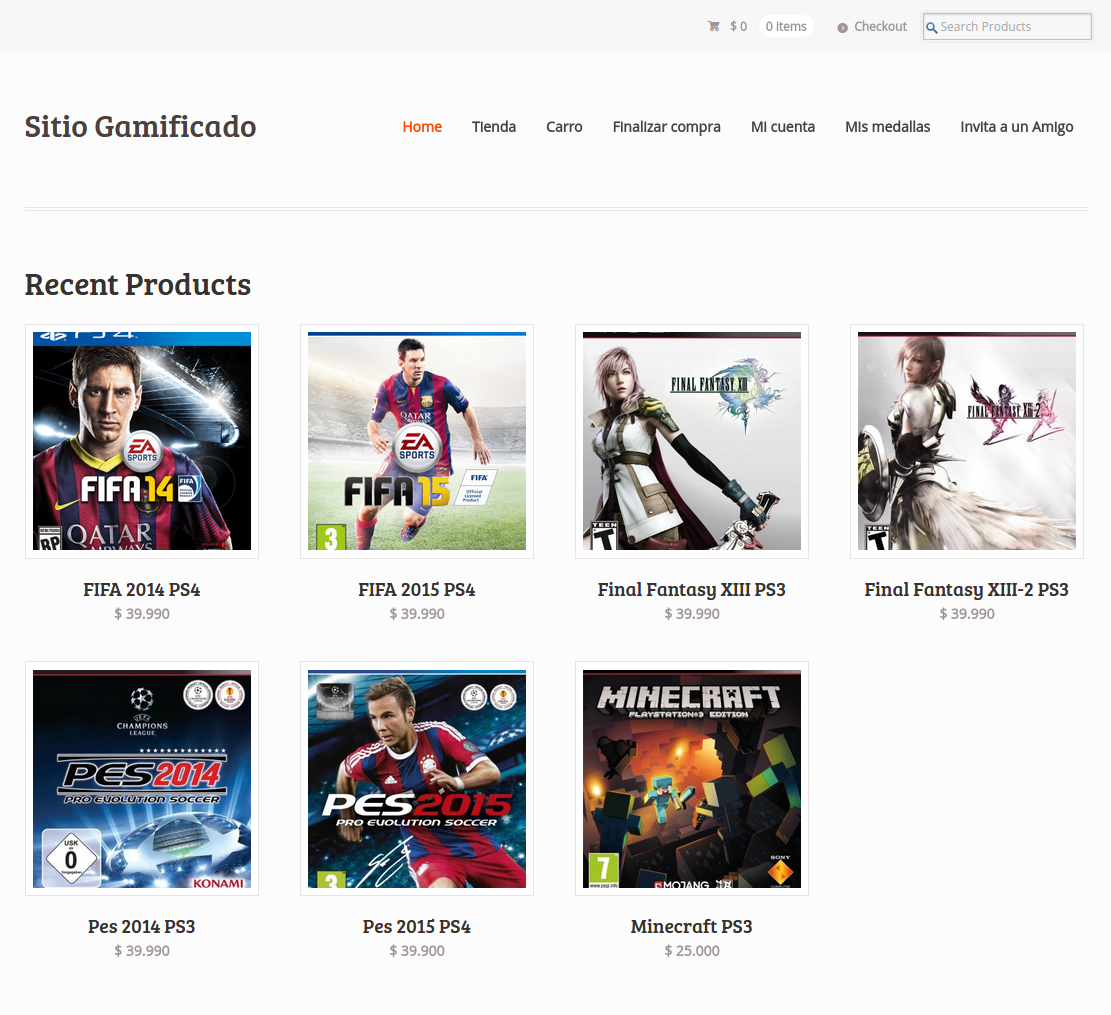
\includegraphics[width=0.9\textwidth]{images/SitioBase.png}
  \caption[TemaVisual]{Tema visual utilizado, vista de la tienda.}
  \label{fig:Players}
\end{figure}



Los plugins utilizados en nuestro sistema, son los siguientes:

\begin{itemize}

    \item {\bf Woocommerce:}
        Es un reconocido módulo que ayuda al usuario a crear una tienda de
        ventas online de forma rápida y sin costo.
        Al ser integrado al sistema, lo modifica agregando opciones
        extra de configuración y administración.
        El uso de éste plugin genera una restricción en la elección
        del tema (\emph{frontend}) del sistema, pues deben ser compatible
        para que exista consistencia en el sitio.
        Dichos temas existen tanto gratuitos como de pago.
        El tema escogido se llama \emph{MyStile}, el cual no posee costo.
        Woocommerce permite administrar de gran forma las características del
        sistema al cual se le pueden agregar una colección de plugins que ayudan a
        aumentar las funcionalidades de este.

    \item {\bf WooCube Pro:}
        Modulo, de pago, encargado de la entrega de puntos a los usuarios luego de
        la realización de las tareas definidas.
        A su vez, es el encargado de dar equivalencia a los puntos así como dar
        validez a estos al ser utilizados como créditos en compras realizadas.
        Este plugin utiliza de base un modulo gratuito, ``Cube points'',
        el cual es la base del diseño de puntaje.
        También incorpora una herramientas para realizar y desplegar una tabla
        de posiciones con los usuarios que han obtenido mayor cantidad de puntaje.

    \item {\bf WPAchievement:}
        Herramienta de pago que entrega la funcionalidad de otorgar achievements,
        logros o medallas a los usuarios luego de realizada alguna de las tareas
        definidas (véase \ref{sec:4.1}).
        Este modulo es el encargado de la entrega de los logros y también del
        guardado de estos para un futuro despliegue de estos.

\begin{figure}[!htb]
  \centering
  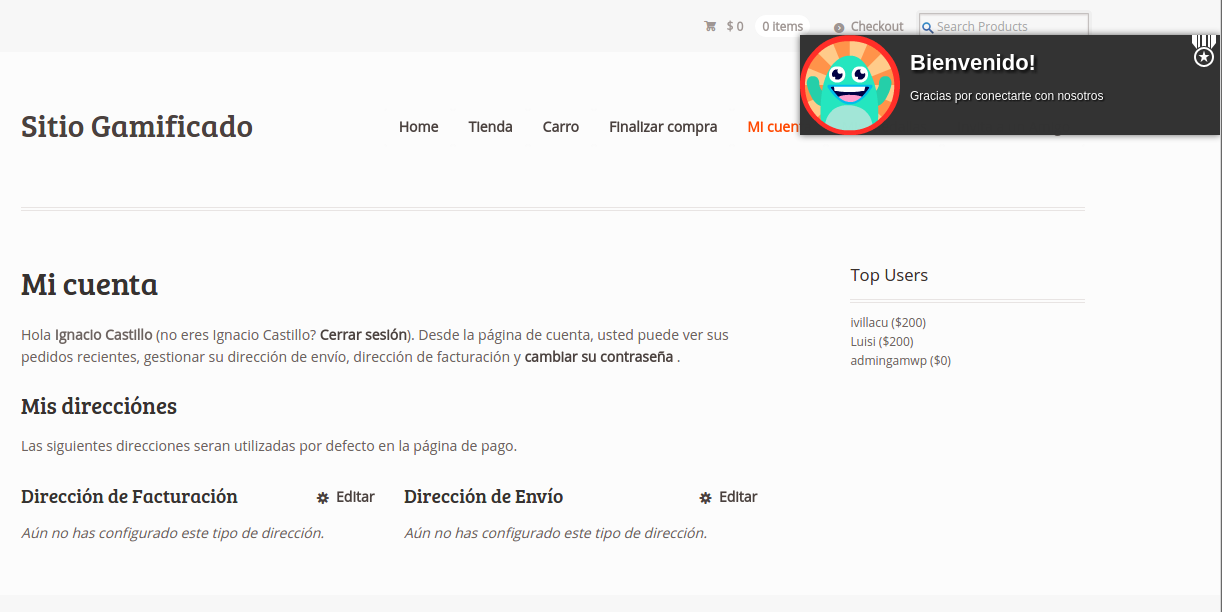
\includegraphics[width=0.8\textwidth]{images/Nuevamedalla.png}
  \caption[achievement]{Entrega de un achievement}
  \label{fig:Players}
\end{figure}

    \item {\bf Refer a Friend:}
        Plugin responsable de la administración de las invitaciones de los
        clientes a potenciales usuarios.
        A su vez se encarga de entregar los beneficios cuando se realiza la tarea
        definida, en el caso de estudio al comprar por primera vez el cliente
        invitado.

\begin{figure}[!htb]
  \centering
  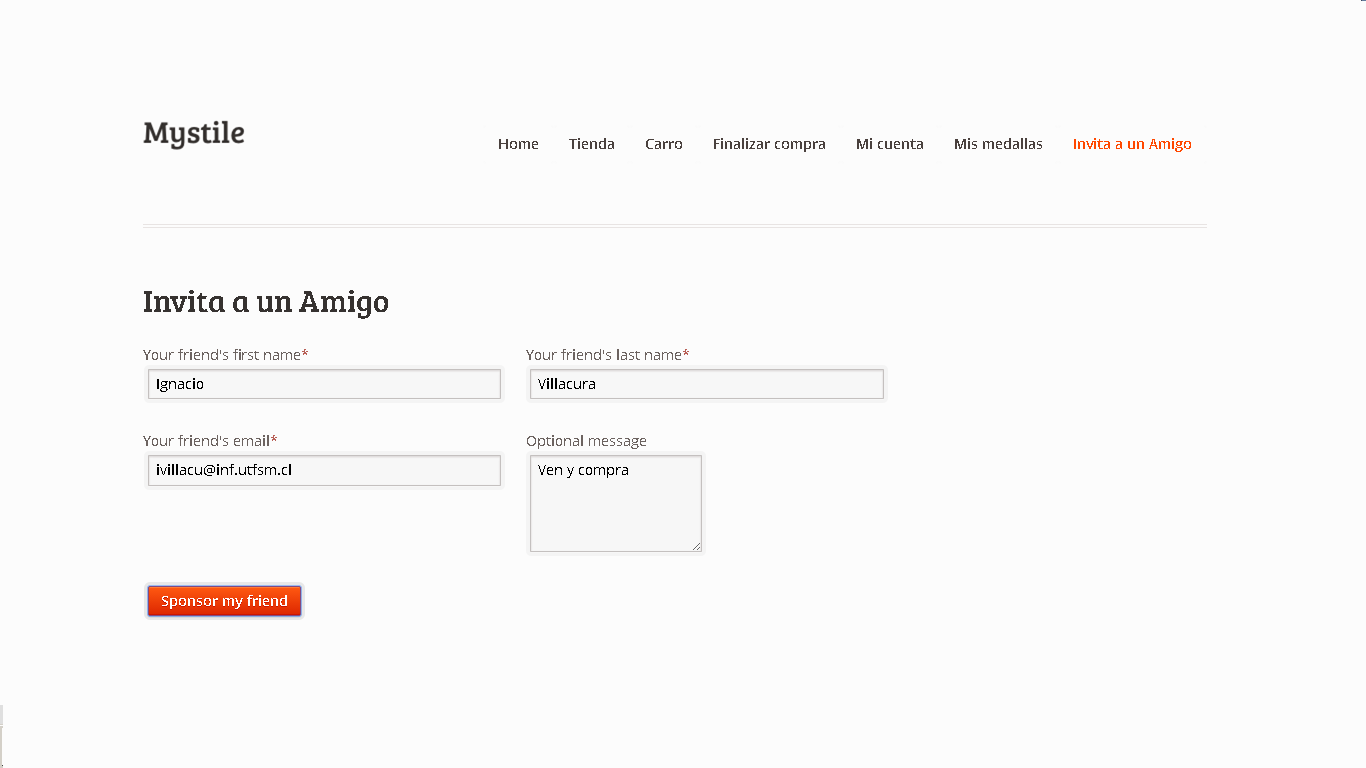
\includegraphics[width=0.8\textwidth]{images/invitaunamigo.png}
  \caption[invitar]{Vista de invitar un amigo}
  \label{fig:Players}
\end{figure}

\end{itemize}

\section{Encuesta evualativa}

Para apoyar el estudio empirico realizado, se creo una encuesta que cuenta con $(x)$ preguntas, con el
objetivo de obtener información mas acabada sobre los gustos de las personas y en especial
si les interesa la idea de utilizar gamification en ventas online. Esta informacion
tambien se puede utilizar para extrapolar ideas sobre la utilizacion de gamification en
ventas prescensiales.

La encuesta tiene como objetivo principal el saber si a la gente, en primer lugar, tiene conocimiento
de que ya han utilizado, de algun modo, gamification ya sea en el supermercado, tiendas de retail,
farmacas, etc. Luego se pregunta si han obtenido o tienen informacion de como obtener alguno
de los beneficios dados en estas tiendas y tambien se les presenta una escala para poder medir
el nivel de aceptacion de beneficios entregados a travez de gamificacion.

A continuacion se explicaran las preguntas con mas sigificado realizadas en la encuesta:
\begin{itemize}
\item Sexo, rango de edad y ocupación: Estos son los datos que nos ayudaran en segmentar
la informacion para ver en que formas se pueden enfocar las herramientas.
\item ¿Esta al tanto de lo que es Gamification?: Pregunta exclusiva para obtener la cantidad de
personas que tienen conocimiento del concepto.
\item ¿Qué beneficios prefiere o preferiría obtener?: Busca encontrar los beneficios que son
 mas interesantes para las personas. Esto ayudara a priorizar beneficios.
\item ¿Cree usted que el uso de Gamificacion lo motiva para volver a comprar en la tienda?: La
base del concepto es que el cliente sea atraido y que vuelva a comprar en la tienda. Esta pregunta
tiene como objetivo encontrar si se crea en las personas la motivación para volver.
\end{itemize}

